
\chapter{Block Diagrams} \label{appendix:Diagram}


This appendix provides a detailed visual representation of the core structural architectures analyzed throughout this project. It includes the comprehensive end-to-end communication block diagram implemented in GNU Radio, highlighting both custom and modified modules, as well as an illustrative example of the rectangular block interleaving matrix performance.

\begin{landscape} % Esto rota la página en el visualizador PDF
    \begin{figure}[p] % Usamos figure normal porque landscape ya rota todo
        \centering
        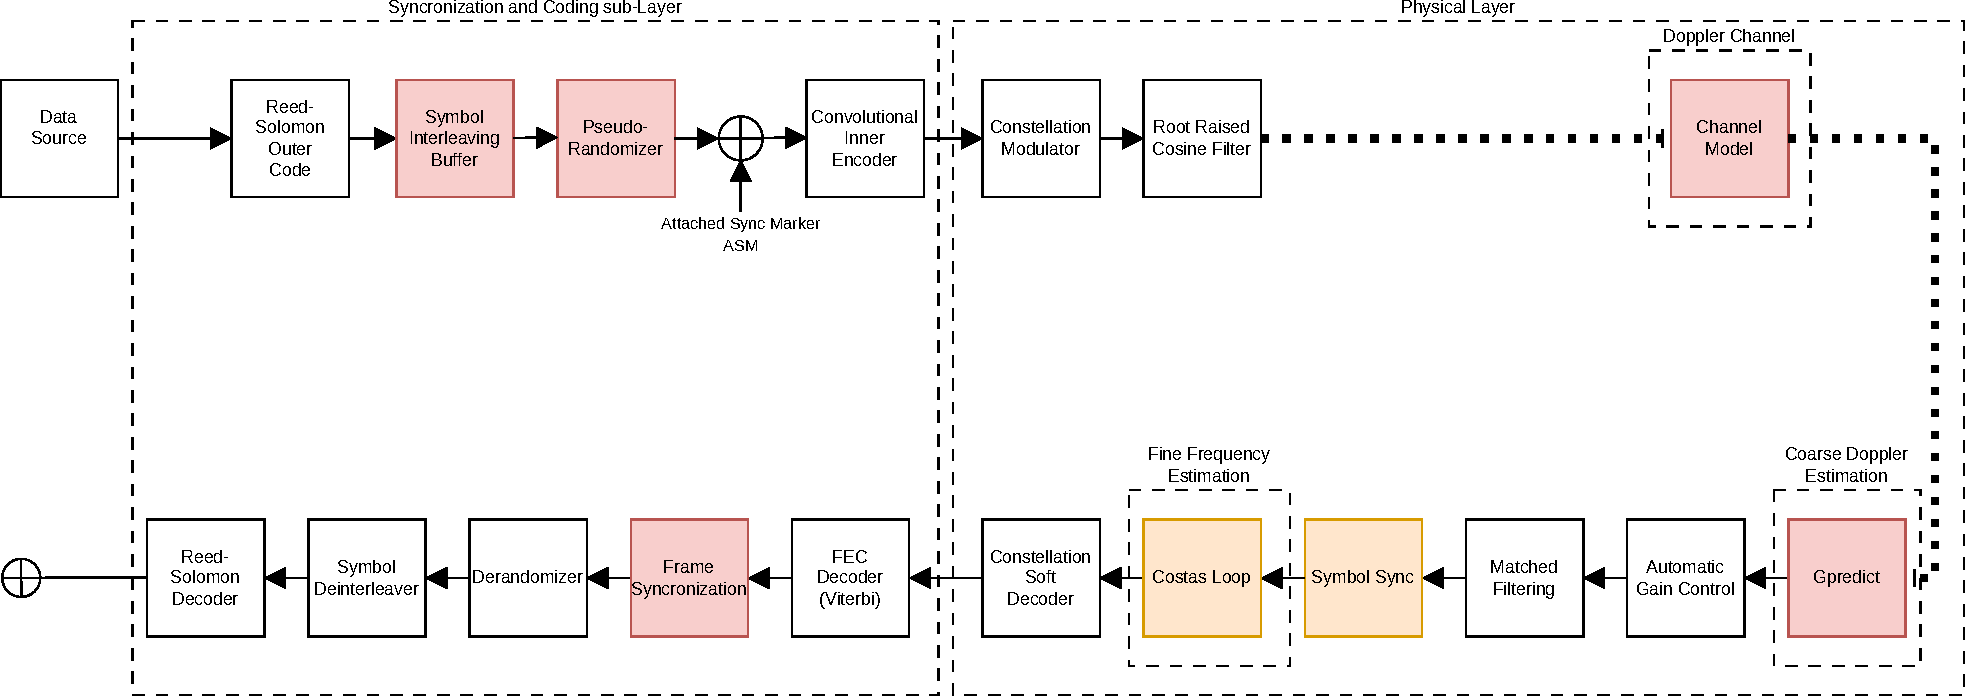
\includegraphics[width=\linewidth]{figures/Inkscape/presentation_red.pdf}
        
    \caption{Complete block diagram of the end-to-end communication system implemented in GNU Radio. Red blocks represent custom DSP modules developed specifically for this project and orange blocks indicate existing library modules that were modified.}
        \label{fig:ccsds_custom}
    \end{figure}
\end{landscape}



\begin{landscape}
    \begin{figure}[p] 
        \centering
        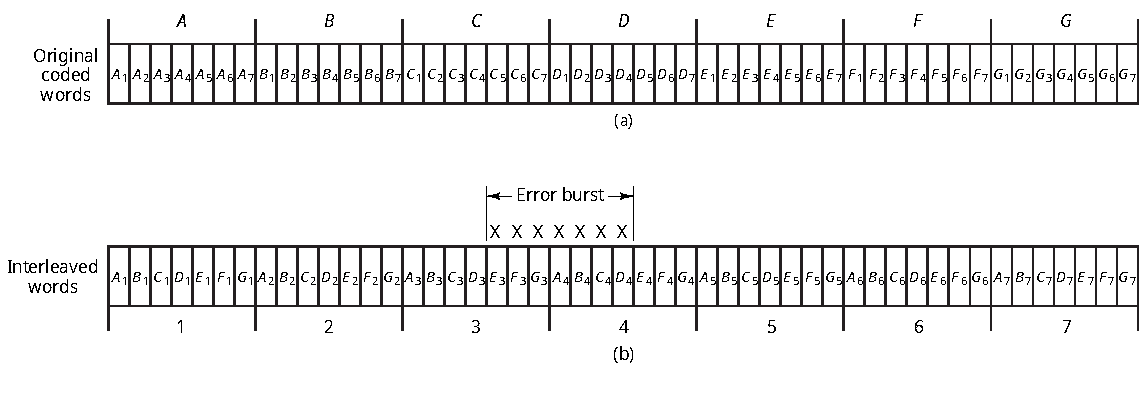
\includegraphics[width=\linewidth]{figures/Inkscape/Interleaver_example_rotated.pdf}
        
        \caption{Interleaving example. (a) Original uninterleaved codewords, each comprised of seven code symbols. (b) Interleaved code symbols.}
        \label{fig:interleaver_example}
    \end{figure}
\end{landscape}